\documentclass[12pt]{ctexart}

\usepackage[margin=2.2cm]{geometry}
\usepackage{amsmath}
\usepackage{booktabs}
\usepackage{tabularx}
\usepackage{enumitem}
\usepackage{titlesec}
\usepackage{xcolor}
\usepackage[hidelinks]{hyperref}
\usepackage{tikz}
\usetikzlibrary{positioning, fit, backgrounds}

\usepackage{xeCJK}
\setmainfont{Liberation Serif}
\setCJKmainfont{Source Han Serif SC}
\setCJKsansfont{Source Han Sans SC}
\setCJKmonofont{Source Han Mono SC}

\definecolor{primary}{RGB}{15,15,35}
\titleformat{\section}{\Large\bfseries\color{primary}}{}{0em}{}
\titlespacing*{\section}{0pt}{1.2em}{0.5em}
\titleformat{\subsection}{\large\bfseries\color{primary}}{}{0em}{}
\titlespacing*{\subsection}{0pt}{0.9em}{0.3em}
\setlist{topsep=0.4em, itemsep=0.2em, parsep=0pt, partopsep=0pt}

\setlength{\parskip}{0.55em}
\setlength{\parindent}{0pt}
\linespread{1.2}

\begin{document}

\pagestyle{empty}

% ===

\begin{center}
  {\LARGE\bfseries AI Agent: Practice}\\[0.35em]
  {\large Week 1 --- LLM and tool-using agent}
\end{center}
\vspace{0.6em}

\section{Agent}

\begin{quote}
\emph{An agent is anything that can be viewed as perceiving its environment through sensors and acting upon that environment through actuators.} --- Russell \& Norvig, \emph{Artificial Intelligence: A Modern Approach}
\end{quote}

\begin{center}
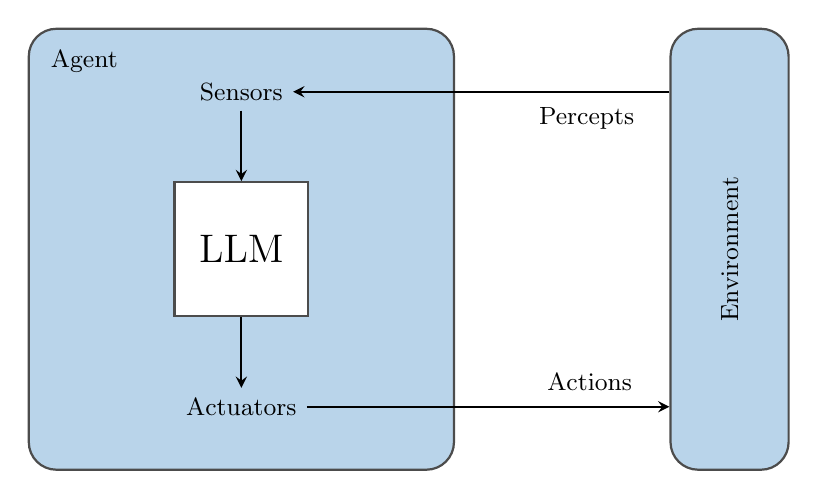
\begin{tikzpicture}[font=\small, >=stealth, thick]
  \definecolor{agentblue}{RGB}{185,212,234}
  \node[draw=black!70, fill=agentblue, rounded corners=10pt, minimum width=5.4cm, minimum height=5.6cm] (agent) at (0,0) {};
  \node[anchor=north west] at (-2.55,2.65) {Agent};
  \node (sensors) at (0,2.0) {Sensors};
  \node[draw=black!70, fill=white, minimum width=1.7cm, minimum height=1.7cm, align=center, font=\Large] (core) at (0,0) {LLM};
  \node (actuators) at (0,-2.0) {Actuators};
  \draw[->] (sensors) -- (core.north);
  \draw[->] (core.south) -- (actuators);
  \node[draw=black!70, fill=agentblue, rounded corners=10pt, minimum width=1.5cm, minimum height=5.6cm] (env) at (6.2,0) {};
  \node[rotate=90] at (6.2,0) {Environment};
  \draw[->] (env.west |- sensors) -- (sensors.east) node[pos=0.22, below=2pt]{Percepts};
  \draw[->] (actuators.east) -- (env.west |- actuators) node[pos=0.78, above=2pt]{Actions};
\end{tikzpicture}
\\[0.3em]
{\small Agents interact with environments through sensors and actuators}
\end{center}

Shrunk to this week, the loop is:

\begin{center}
\begin{tabularx}{0.94\textwidth}{@{}l X@{}}
  \toprule
  \textbf{Loop element} & \textbf{This week it is} \\
  \midrule
  Environment & user requests and tools to call                 \\
  Percepts    & the transcript so far and each new tool result  \\
  Actions     & a tool call, or the final answer                \\
  Reward      & the spec below (pass/fail scenarios)            \\
  \bottomrule
\end{tabularx}
\end{center}

\begin{center}
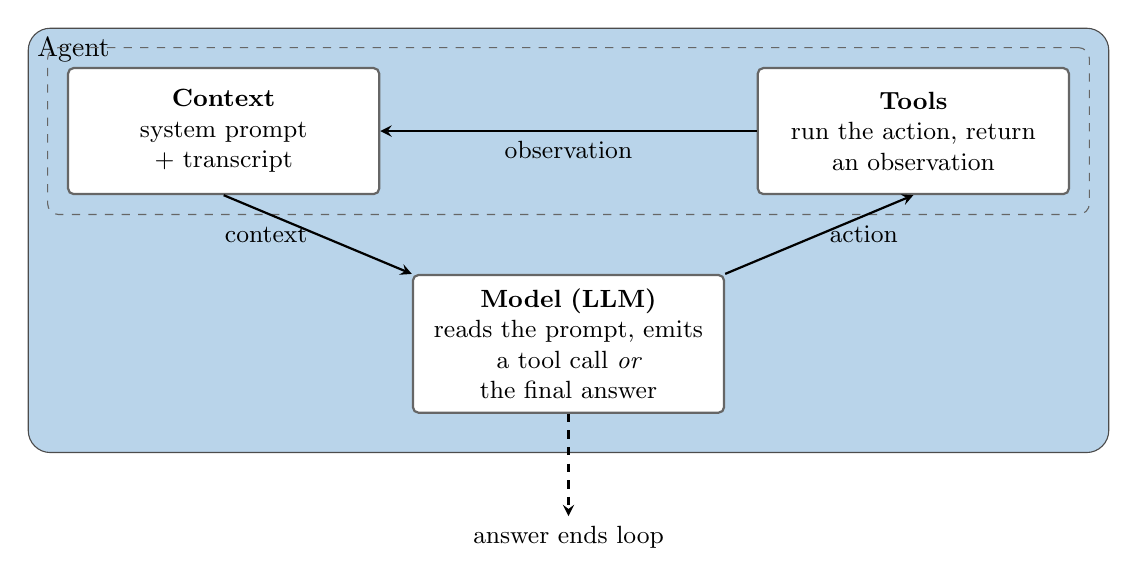
\begin{tikzpicture}[font=\small, >=stealth, thick,
  box/.style={draw=black!60, rounded corners=2pt, align=center, inner sep=5pt, text width=3.6cm, minimum height=1.6cm, fill=white}]
  \definecolor{agentblue}{RGB}{185,212,234}
  \node[box] (llm) {\textbf{Model (LLM)}\\ reads the prompt, emits\\ a tool call \emph{or} the final answer};
  \node[box, above left=1.0cm and 0.4cm of llm] (hist) {\textbf{Context}\\ system prompt + transcript};
  \node[box, above right=1.0cm and 0.4cm of llm] (tools) {\textbf{Tools}\\ run the action, return\\ an observation};
  \draw[->] (hist.south) -- node[left, midway]{context} (llm.north west);
  \draw[->] (llm.north east) -- node[right, midway]{action} (tools.south);
  \draw[->] (tools.west) -- node[below, midway]{observation} (hist.east);
  \draw[->,dashed] (llm.south) -- ++(0,-1.3) node[below]{answer ends loop};
  \begin{scope}[on background layer]
    \node[draw=black!70, rounded corners=8pt, fill=agentblue, fit=(llm)(hist)(tools), inner sep=14pt,
      label={[anchor=north west, font=\normalsize]north west:Agent}] (agentbox) {};
    \node[draw=black!60, dashed, rounded corners=4pt, fit=(hist)(tools), inner sep=7pt,
      label={[anchor=north west, xshift=8pt, yshift=-5pt, font=\small\bfseries]north west:Harness}] (harness) {};
  \end{scope}
\end{tikzpicture}
\\[0.3em]
{\small Agent = model + harness}
\end{center}

ReAct (\href{https://arxiv.org/abs/2210.03629}{Yao et al.\ 2022}): Thought, Action, Observation.

\section{LLM: the decision-maker}

The decision-maker inside the loop above is a \emph{LLM} (\strong{L}arge \strong{L}anguage \strong{M}odel). It reads a sequence of tokens and predicts the next one.

\subsection{Tokens}

The input of LLM are \emph{Token}s, encompassing text, images, and videos (multimodal).

\subsection{Pricing}

Expanding:

\url{https://api-docs.deepseek.com/quick_start/pricing/}

\url{https://developers.openai.com/api/docs/pricing}

\subsection{Context window}

In token, e.g. $ 40960 = 40 \times 1024 $

\subsection{Latency}

\begin{description}
  \item[TTFT] Time to First Token
  \item[TPS]  Tokens per Second
\end{description}

\subsection{Real world Model}

Run ollama show qwen3:8b

\begin{verbatim}
  Model
    architecture        qwen3     
    parameters          8.2B      
    context length      40960     
    embedding length    4096      
    quantization        Q4_K_M    

  Capabilities
    completion    
    tools         
    thinking      

  Parameters
    repeat_penalty    1                 
    stop              "<|im_start|>"    
    stop              "<|im_end|>"      
    temperature       0.6               
    top_k             20                
    top_p             0.95              

  License
    Apache License               
    Version 2.0, January 2004    
\end{verbatim}
    ...

\section{The harness}

All but Model itself.

\section{Tool calling}

Expanding:

\url{https://api-docs.deepseek.com/guides/tool_calls}

\begin{verbatim}
{ "type": "function",
  "function": { "name": "get_weather",
                "description": "Today's temperature (Celsius) in a city.",
                "parameters": { "type": "object",
                                "properties": {"city": {"type": "string"}},
                                "required": ["city"] } } }
\end{verbatim}

\subsection{How a round trip is marked}

\begin{center}
\begin{tabular}{@{}l@{\quad}l@{}}
  \texttt{system} & fixed instructions we control \\
  \texttt{user} & the request \\
  \texttt{assistant} & the model's turn: text, or a tool call \\
  \texttt{tool} & the result of one call, linked to the call it answers \\
\end{tabular}
\end{center}

Example.

\begin{verbatim}
system     "You are a minimal ReAct agent..."
user       What is the weather in Tokyo?
assistant  tool call: get_weather(city: "Tokyo")
tool       Tokyo: 18 °C
assistant  It is 18 °C in Tokyo right now.
\end{verbatim}

\section{The spec it must pass}

\textbf{[TODO]}

\section{Lab}

\textbf{[TODO --- hands-on under design.]}

\noindent\textbf{Next week:} tools in depth --- schemas worth writing, errors a model can recover from, safety.

\end{document}
